\documentclass[14pt]{extarticle}
\usepackage{fontspec}
\usepackage{polyglossia}
\usepackage{amsmath}
\usepackage{amssymb}
\usepackage{xcolor}
\usepackage{fancyhdr}
\usepackage{graphicx}
\usepackage{listings}
\usepackage[most]{tcolorbox}
% \usepackage{setspace}
\usepackage{pifont}
\usepackage{enumitem}
\usepackage{titlesec}
\usepackage[bottom]{footmisc}
\usepackage{titling}
\usepackage{minted}
\usepackage{etoolbox}
\usepackage{array}
\usepackage{extsizes}
\usepackage{float}
\usepackage{booktabs}
\usepackage{hyperref}
\usepackage[onehalfspacing]{setspace}
\usepackage[a4paper, top=2.7cm, bottom=2.7cm, left=2.5cm, right=2.5cm, headheight=1.5cm, headsep=0.5cm]{geometry}
\usepackage{tikz}

\usetikzlibrary{automata, positioning, arrows.meta, arrows}

\newfontfamily\emoji{Segoe UI Emoji}

\pagestyle{fancy}

\setmainlanguage[numerals=western]{arabic}
\setotherlanguage{english}
% \newfontfamily\arabicfont[Script=Arabic]{Amiri}
\newfontfamily\arabicfont[Script=Arabic]{Calibri}
\newfontfamily\arabicfonttt[Script=Arabic]{Courier New}

\lstset{
  language=[Sharp]C,
  numbers=left,
  stepnumber=1,
  numbersep=8pt,
  frame=single,
  basicstyle=\ttfamily\small,
  keywordstyle=\color{blue},
  stringstyle=\color{red},
  commentstyle=\color{green!50!black}
}

\newif\ifdetailed
\ifdefined\setdetailed
  \setdetailed
\fi

\newif\ifwithsols
\ifdefined\setwithsols
  \setwithsols
\fi

% unified tcolorboxes for articles
\tcbset{colback=white, colframe=black, fonttitle=\bfseries, boxrule=0.8pt}
\newtcolorbox{boxDef}[1][]{colback=blue!5!white,colframe=blue!75!black,
  title={{\emoji📘} تعريف\ifx\\#1\\\else ~#1\fi :}}
\newtcolorbox{boxExercise}[1][]{colback=cyan!5!white,colframe=cyan!70!black,
  title={{\emoji🧩} تمرين\ifx\\#1\\\else ~#1\fi :}}
\newtcolorbox{boxExample}[1][]{colback=yellow!5!white,colframe=orange!90!black,
  title={{\emoji📝} مثال\ifx\\#1\\\else ~#1\fi :}}
\newtcolorbox{boxNote}[1][]{colback=gray!10!white,colframe=black,
  title={{\emoji✨} ملاحظة\ifx\\#1\\\else ~#1\fi :}}
\newtcolorbox{boxAttention}[1][]{colback=magenta!10!white,colframe=magenta!80!black,
  title={{\emoji🔔} تنبيه\ifx\\#1\\\else ~#1\fi :}}
\newtcolorbox{boxWarning}[1][]{colback=red!5!white,colframe=red!75!black,
  title={{\emoji⚡} ملاحظة هامة\ifx\\#1\\\else ~#1\fi :}}
\newtcolorbox{boxSolution}[1][]{colback=green!5!white,colframe=green!60!black,
  title={{\emoji✅} حل\ifx\\#1\\\else ~#1\fi :}}
\newtcolorbox{boxSymbol}[1][]{colback=purple!5!white,colframe=purple!70!black,
  title={{\emoji🔣} رمز\ifx\\#1\\\else ~#1\fi :}}
\newtcolorbox{boxHint}[1][]{colback=teal!5!white,colframe=teal!60!black,
  title={{\emoji💡} تلميح\ifx\\#1\\\else ~#1\fi :}}


\tcbset{simplecode/.style={ colback=gray!5, colframe=black!50, boxrule=0.4pt, arc=2pt, left=4pt,right=4pt,top=4pt,bottom=4pt}}
\newenvironment{boxCode}{\begin{tcolorbox}[simplecode]}{\end{tcolorbox}}

\newcolumntype{C}[1]{>{\centering\arraybackslash}p{#1}}

% redefine spaces after titles
\makeatletter
\renewcommand{\@maketitle}{%
  \begin{center}
    {\huge \bfseries \@title \par}%
    \vskip 0.2em % space between title and author
    {\large \@author \par}%
    % \vskip 0.2em % space between author and date
    % {\normalsize \@date \par}%
  \end{center}
}
\makeatother

\fancyhf{} % clear default
\fancypagestyle{plain}{
  \fancyhf{}
  \fancyhead[L]{مدرسة التسامح الشاملة}
  % \fancyhead[L]{
\includegraphics[height=1cm]{../../../images/logoTasamoh.png}}
  \fancyhead[R]{الأستاذ محمود اغبارية}
  \fancyfoot[C]{\thepage}
}

\fancyhead[L]{مدرسة التسامح الشاملة}
\fancyhead[R]{الأستاذ محمود اغبارية}
\fancyfoot[C]{\thepage}
% \date{\today}

\setcounter{tocdepth}{3} % only section subsection and subsubsection in TOC

\newcommand{\importpdfpage}[2]{%
    \thispagestyle{empty}
    \newgeometry{left=0cm,right=0cm,top=0cm,bottom=0cm}
    \includegraphics[page=#2,width=0.95\paperwidth,height=0.95\paperheight,keepaspectratio]{#1}
    \restoregeometry
}

\newcommand{\insertFullImg}[1]{%
    \noindent
    \makebox[\textwidth][c]{
        \includegraphics[width=0.9\paperwidth,keepaspectratio]{#1}%
    }%
}%

% ----------------------


% \begin{document}

% \maketitle

% % \clearpage  % start TOC on a new page
% % \renewcommand{\contentsname}{جدول المحتويات}
% % \tableofcontents
% % \clearpage

% \part*{part 1} % the * prevents numbering
% \section*{مقدمة}
% \subsection*{مثال رياضي}
% \subsubsection*{مثال فرعي}
% \paragraph*{ paragraph 1}
% \subparagraph*{sub paragraph 1}

% \ifdetailed
% \begin{english}
% \begin{minted}{csharp}
% // C# Example
% \end{minted}
% \end{english}
% \fi

% OLD WAY
% \ifdetailed
% \begin{english}
% \begin{lstlisting}
% // C# Example
% \end{lstlisting}
% \end{english}
% \fi

% % 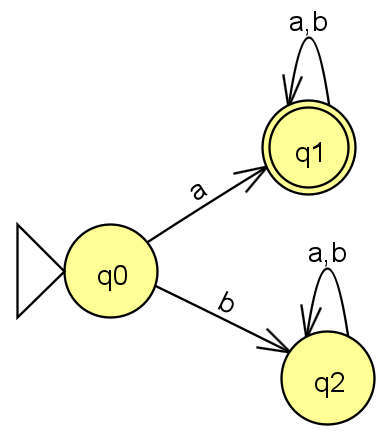
\includegraphics[width=0.2\textwidth]{../../../images/DFAs/ex1_q1.png}



% \vspace{3cm}
% \begin{flushleft}
% أرجو لكم وقتًا ممتعًا.

% الأستاذ محمود اغبارية.
% \end{flushleft}


% \end{document}


\ifwithsols
\title{حل ورقة تمرّن 19 \\ مصفوفة كائنات + فئات مع مصفوفة}
\else
\title{ورقة تمرّن 19 \\ مصفوفة كائنات + فئات مع مصفوفة}
\fi

\begin{document}

\maketitle
\thispagestyle{fancy}

%=============================================================
\section{مصفوفة كائنات}
%=============================================================

تستخدم هذه الأسئلة الفئة \textenglish{Car} التالية:

\begin{boxExample}
\begin{english}
{\small
\begin{minted}{csharp}
class Car
{
    private string Brand;
    private int    Year;
    private double Price;

    public Car(string brand, int year, double price)
    {
        this.Brand = brand;
        this.Year  = year;
        this.Price = price;
    }

    public string GetBrand() { return Brand; }
    public int    GetYear()  { return Year;  }
    public double GetPrice() { return Price; }

    public void SetPrice(double p) { if (p > 0) Price = p; }

    public bool IsNew() { return Year >= 2022; }

    public void Print()
    {
        Console.WriteLine($"{Brand} ({Year}) - {Price} NIS");
    }
}
\end{minted}
}
\end{english}
\end{boxExample}

\begin{enumerate}

\clearpage
%--- سؤال 1.1 ---
\item
عرِّف في \textenglish{Main} مصفوفة \textenglish{cars} من نوع \textenglish{Car} بحجم 3،
واملأها بالبيانات التالية، ثم اطبع جميع السيارات:

\begin{center}
\begin{tabular}{|c|c|c|}
\hline
\textbf{الماركة} & \textbf{السنة} & \textbf{السعر} \\
\hline
\textenglish{Toyota} & \textenglish{2021} & \textenglish{80000} \\
\textenglish{Honda}  & \textenglish{2023} & \textenglish{95000} \\
\textenglish{Kia}    & \textenglish{2019} & \textenglish{65000} \\
\hline
\end{tabular}
\end{center}

\ifwithsols
\begin{boxSolution}
\begin{english}
{\small
\begin{minted}{csharp}
// In Main
Car[] cars = new Car[3];
cars[0] = new Car("Toyota", 2021, 80000);
cars[1] = new Car("Honda",  2023, 95000);
cars[2] = new Car("Kia",    2019, 65000);

for (int i = 0; i < cars.Length; i++)
    cars[i].Print();
\end{minted}
}
\end{english}
\end{boxSolution}
\clearpage
\fi

%--- سؤال 1.2 ---
\item
بافتراض وجود المصفوفة \textenglish{cars}، اكتب كودًا يطبع فقط السيارات الجديدة
(باستخدام العملية \textenglish{IsNew()}).

\ifwithsols
\begin{boxSolution}
\begin{english}
{\small
\begin{minted}{csharp}
// In Main
for (int i = 0; i < cars.Length; i++)
{
    if (cars[i].IsNew())
        cars[i].Print();
}
\end{minted}
}
\end{english}
\end{boxSolution}
\clearpage
\fi

%--- سؤال 1.3 ---
\item
بافتراض وجود المصفوفة \textenglish{cars}، اكتب كودًا يحسب ويطبع مجموع أسعار
جميع السيارات.

\ifwithsols
\begin{boxSolution}
\begin{english}
{\small
\begin{minted}{csharp}
// In Main
double total = 0;
for (int i = 0; i < cars.Length; i++)
    total += cars[i].GetPrice();

Console.WriteLine("Total: " + total + " NIS");
\end{minted}
}
\end{english}
\end{boxSolution}
\clearpage
\fi

%--- سؤال 1.4 ---
\item
بافتراض وجود المصفوفة \textenglish{cars}، اكتب كودًا يجد السيارة الأرخص ويطبعها.

\ifwithsols
\begin{boxSolution}
\begin{english}
{\small
\begin{minted}{csharp}
// In Main
Car cheapest = cars[0];
for (int i = 1; i < cars.Length; i++)
{
    if (cars[i].GetPrice() < cheapest.GetPrice())
        cheapest = cars[i];
}

Console.Write("Cheapest: ");
cheapest.Print();
\end{minted}
}
\end{english}
\end{boxSolution}
\clearpage
\fi

%--- سؤال 1.5 ---
\item
اكتب عملية خارجية (\textenglish{static}) باسم \textenglish{GetAffordable}
تتلقى مصفوفة \textenglish{Car[]} وعددًا \textenglish{double budget}،
وتُعيد مصفوفة جديدة تحتوي فقط السيارات التي سعرها أقل من أو يساوي \textenglish{budget}.

ثم استدعِها في \textenglish{Main} بميزانية \textenglish{85000} واطبع النتيجة.

\ifwithsols
\begin{boxSolution}
\begin{english}
{\small
\begin{minted}{csharp}
public static Car[] GetAffordable(Car[] cars, double budget)
{
    int count = 0;
    for (int i = 0; i < cars.Length; i++)
        if (cars[i].GetPrice() <= budget)
            count++;

    Car[] result = new Car[count];
    int j = 0;
    for (int i = 0; i < cars.Length; i++)
    {
        if (cars[i].GetPrice() <= budget)
        {
            result[j] = cars[i];
            j++;
        }
    }
    return result;
}

// In Main
Car[] affordable = GetAffordable(cars, 85000);
for (int i = 0; i < affordable.Length; i++)
    affordable[i].Print();
\end{minted}
}
\end{english}
\end{boxSolution}
\fi

\end{enumerate}

\clearpage
%=============================================================
\section{فئة تحتوي على مصفوفة كخاصية}
%=============================================================

تستخدم هذه الأسئلة الفئة \textenglish{Player} التالية:

\begin{boxExample}
\begin{english}
{\small
\begin{minted}{csharp}
class Player
{
    private string Name;
    private int[]  Scores; // scores in each game

    public Player(string name, int[] scores)
    {
        this.Name   = name;
        this.Scores = scores;
    }

    public string GetName()   { return Name;   }
    public int[]  GetScores() { return Scores; }

    public void Print()
    {
        Console.Write(Name + ": ");
        for (int i = 0; i < Scores.Length; i++)
            Console.Write(Scores[i] + " ");
        Console.WriteLine();
    }
}
\end{minted}
}
\end{english}
\end{boxExample}

\begin{enumerate}

%--- سؤال 2.1 ---
\item
أنشئ في \textenglish{Main} كائنَين من نوع \textenglish{Player} بالبيانات التالية
واطبع كل منهما:

\begin{center}
\begin{tabular}{|c|l|}
\hline
\textbf{الاسم} & \textbf{النقاط} \\
\hline
\textenglish{Ali}  & \textenglish{10, 20, 15} \\
\textenglish{Rami} & \textenglish{8, 25, 12, 18} \\
\hline
\end{tabular}
\end{center}

\ifwithsols
\begin{boxSolution}
\begin{english}
{\small
\begin{minted}{csharp}
// In Main
int[] s1 = { 10, 20, 15 };
Player p1 = new Player("Ali", s1);

int[] s2 = { 8, 25, 12, 18 };
Player p2 = new Player("Rami", s2);

p1.Print();
p2.Print();
\end{minted}
}
\end{english}
\end{boxSolution}
\clearpage
\fi

%--- سؤال 2.2 ---
\item
أضِف إلى الفئة \textenglish{Player} عملية \textenglish{GetTotal()} تُعيد مجموع نقاطه
في كل المباريات.
ثم استدعِها في \textenglish{Main} واطبع المجموع لكلا اللاعبَين.

\ifwithsols
\begin{boxSolution}
\begin{english}
{\small
\begin{minted}{csharp}
// Inside class Player
public int GetTotal()
{
    int sum = 0;
    for (int i = 0; i < Scores.Length; i++)
        sum += Scores[i];
    return sum;
}

// In Main
Console.WriteLine(p1.GetName() + " total: " + p1.GetTotal());
Console.WriteLine(p2.GetName() + " total: " + p2.GetTotal());
\end{minted}
}
\end{english}
\end{boxSolution}
\clearpage
\fi

%--- سؤال 2.3 ---
\item
أضِف إلى الفئة \textenglish{Player} عملية \textenglish{GetBest()} تُعيد أعلى نقطة
حصل عليها اللاعب في مباراة واحدة.
ثم استدعِها في \textenglish{Main} واطبع النتيجة لكلا اللاعبَين.

\ifwithsols
\begin{boxSolution}
\begin{english}
{\small
\begin{minted}{csharp}
// Inside class Player
public int GetBest()
{
    int best = Scores[0];
    for (int i = 1; i < Scores.Length; i++)
        if (Scores[i] > best)
            best = Scores[i];
    return best;
}

// In Main
Console.WriteLine(p1.GetName() + " best: " + p1.GetBest());
Console.WriteLine(p2.GetName() + " best: " + p2.GetBest());
\end{minted}
}
\end{english}
\end{boxSolution}
\clearpage
\fi

%--- سؤال 2.4 ---
\item
أضِف إلى الفئة \textenglish{Player} عملية \textenglish{GetAverage()} تُعيد متوسط نقاطه.
ثم أضِف عملية \textenglish{IsBetter(Player other)} تُعيد \textenglish{true} إذا كان
متوسط هذا اللاعب أعلى من متوسط اللاعب الآخر.

استخدمها في \textenglish{Main} لطباعة اسم اللاعب الأفضل من الاثنين.

\ifwithsols
\begin{boxSolution}
\begin{english}
{\small
\begin{minted}{csharp}
// Inside class Player
public double GetAverage()
{
    return (double)GetTotal() / Scores.Length;
}

public bool IsBetter(Player other)
{
    return this.GetAverage() > other.GetAverage();
}

// In Main
if (p1.IsBetter(p2))
    Console.WriteLine(p1.GetName() + " is better.");
else
    Console.WriteLine(p2.GetName() + " is better.");
\end{minted}
}
\end{english}
\end{boxSolution}
\clearpage
\fi

%--- سؤال 2.5 ---
\item
أضِف إلى الفئة \textenglish{Player} عملية بنّاءة ثانية تتلقى الاسم فقط
وتُهيّئ مصفوفة نقاط فارغة بحجم \textenglish{5} (جميع قيمها صفر).

ثم أضِف عملية \textenglish{SetScore(int index, int value)} تُعيّن نقطة
في مباراة معيّنة (تحقّق أن \textenglish{index} ضمن الحدود وأن \textenglish{value >= 0}).

اختبِر في \textenglish{Main} بإنشاء لاعب بالاسم فقط ثم تعيين نقاطه واحدة واحدة وطباعته.

\ifwithsols
\begin{boxSolution}
\begin{english}
{\small
\begin{minted}{csharp}
// Inside class Player — second constructor
public Player(string name)
{
    this.Name   = name;
    this.Scores = new int[5]; // all zeros by default
}

// Inside class Player — SetScore
public void SetScore(int index, int value)
{
    if (index >= 0 && index < Scores.Length && value >= 0)
        Scores[index] = value;
}

// In Main
Player p3 = new Player("Sami");
p3.SetScore(0, 14);
p3.SetScore(1, 22);
p3.SetScore(2, 9);
p3.SetScore(3, 17);
p3.SetScore(4, 11);
p3.Print();
\end{minted}
}
\end{english}
\end{boxSolution}
\fi

\end{enumerate}

\vspace{1em}
\begin{flushleft}
أرجو لكم عملاً ممتعاً!

الأستاذ محمود اغبارية
\end{flushleft}

\end{document}
